\documentclass[12pt]{article}

\usepackage[margin=1in]{geometry}
\usepackage{hyperref}
\usepackage{booktabs}
\usepackage{graphicx}
\graphicspath{{results/20260423_033257_workload_sweep_azure/figures/}}
\usepackage{amsmath}
\usepackage{enumitem}
\usepackage{parskip}
\usepackage{microtype}
\usepackage{caption}
\usepackage{float}
\usepackage{listings}
\usepackage{xcolor}

\hypersetup{colorlinks=true, linkcolor=blue, urlcolor=blue, citecolor=blue}

\lstset{
  basicstyle=\ttfamily\small,
  breaklines=true,
  frame=single,
  backgroundcolor=\color{gray!10},
}

\title{\textbf{Design and Evaluation of a Cross-Region Intelligent Load Balancer\\
for Latency--Load Tradeoffs}\\[0.5em]
\large Spring 2026 CS640 Final Project Report\\
University of Wisconsin-Madison}

\author{Stefan Arsov \quad Zach Zemanovic\\
\small\texttt{sarsov@wisc.edu} \quad \texttt{zemanovic@wisc.edu}}

\date{May 5, 2026}

\begin{document}

\maketitle

% ─────────────────────────────────────────────────────────────────────────────
\begin{abstract}
Modern distributed applications are deployed across geographically dispersed
compute resources, where load balancers determine how client requests are
routed. Traditional strategies such as round-robin or lowest-latency routing
are uninformed about backend compute state, which can lead to suboptimal
tail latency and throughput when backends are heterogeneous or asymmetrically
loaded. This paper presents \textbf{inteliLB}, an HTTP load balancer
implemented in Go that supports six routing algorithms — round-robin,
least-connections, lowest-latency, lowest-CPU, intelligent (static
multi-metric weighted scoring), and adaptive (dynamically reweighted
multi-metric scoring) — and evaluates them against asymmetric Azure VM
backends across three geographic regions. We ran five workload profiles
(CPU-only, high-connection, I/O-bound, bimodal, and realistic mixed) and a
calibrated open-loop saturation ramp. Our results show that
\textbf{least-connections outperforms all algorithms} on CPU-bound and mixed
workloads, achieving up to 40\% higher throughput than round-robin and 2$\times$
higher throughput on connection-heavy profiles. Latency-based routing exhibits
a strong network proximity bias that overrides compute capacity signals, routing
96\% of traffic to the weakest backend. The adaptive algorithm shows promise
but is hampered by a cold-start window and a 30-second weight recomputation
cycle that introduces mid-run routing shifts. We discuss the design, the
experimental methodology, and directions for future work.

\vspace{0.5em}
\noindent\textbf{Git repository:}
\url{https://github.com/zemanovic/inteliLB}
\end{abstract}

\tableofcontents
\newpage

% ─────────────────────────────────────────────────────────────────────────────
\section*{General Information}
\begin{itemize}[leftmargin=2em]
  \item \textbf{Names:} Stefan Arsov, Zach Zemanovic
  \item \textbf{Emails:} \texttt{sarsov@wisc.edu}, \texttt{zemanovic@wisc.edu}
  \item \textbf{Home department:} Computer Sciences
  \item \textbf{Status:} MS Students
  \item \textbf{Teammate note:} Both team members contributed to this report;
        the reports are not identical but cover the same experimental work.
  \item \textbf{Open source:} We release the inteliLB source code as open
        source under a BSD3 license for unfettered use by any interested party.
\end{itemize}

% ─────────────────────────────────────────────────────────────────────────────
\section{Problem Statement}

Load balancers are a foundational component of distributed systems, responsible
for distributing client requests across a pool of backend servers. In modern
cloud deployments, those backends are rarely homogeneous: different VM sizes,
different geographic regions, and different instantaneous load levels mean that
a routing decision that ignores compute state will systematically over-utilize
some backends while under-utilizing others.

The standard textbook approaches handle this poorly. Round-robin distributes
requests uniformly regardless of backend capacity or health. Lowest-latency
routing minimizes network round-trip time but conflates network proximity with
compute availability — a backend that is geographically close may be heavily
loaded. Single-metric policies (lowest CPU, least connections) capture one
dimension of backend state but miss the others.

The motivating scenario for this project is a client with low network latency
to \textbf{Region A} running at 90\% CPU utilization, and moderate latency to
\textbf{Region B} with ample available compute. A latency-based router sends
the request to Region A, where it queues behind saturated workers. An
intelligent router that weighs both network latency and compute availability
may route to Region B, accepting a small RTT penalty in exchange for a large
reduction in queueing delay, yielding lower overall response time.

\textbf{Research question:} Do multi-metric routing strategies (intelligent,
adaptive) meaningfully outperform single-metric and round-robin baselines
when backends are asymmetric in compute capacity and geographic distance,
under a range of workload types and offered loads?

\textbf{Hypothesis:} Multi-metric intelligent routing will reduce tail latency
and improve throughput stability over single-metric and round-robin approaches,
particularly under CPU-heavy asymmetric load.

% ─────────────────────────────────────────────────────────────────────────────
\section{Solution Description}

\subsection{System Architecture}

inteliLB is a pure-Go HTTP reverse proxy that sits between a client and a pool
of backend servers. The load balancer runs locally; backends are remote Azure
VMs. The overall data path is:

\begin{center}
\texttt{Client $\longrightarrow$ inteliLB (local) $\longrightarrow$
Backend-N (Azure, cross-region)}
\end{center}

The balancer exposes two endpoints to the client: \texttt{/work} (proxied to a
backend) and \texttt{/lb/stats} (JSON snapshot of per-backend metrics and
request counts). A hot-swap REST endpoint (\texttt{POST /lb/algorithm}) allows
the active routing algorithm to be changed without restarting the process.

\subsection{Backend Infrastructure}

Three Azure VMs were deployed across distinct geographic regions to produce
heterogeneous network latency and compute capacity:

\begin{table}[H]
\centering
\begin{tabular}{llll}
\toprule
Backend & Region & VM SKU & Effective vCPUs \\
\midrule
backend-1 & westus2 (Washington) & Standard\_D2s\_v3 & 1 (taskset pinned) \\
backend-2 & northcentralus (Illinois) & Standard\_D2s\_v3 & 2 \\
backend-3 & eastus2 (Virginia) & Standard\_D4s\_v3 & 4 \\
\bottomrule
\end{tabular}
\caption{Azure backend layout. backend-1 is the closest region to the test
client and the weakest in compute; backend-3 is the most distant and most
powerful.}
\end{table}

Each backend runs a Go HTTP server (\texttt{cmd/backend}) that handles two
request types:
\begin{itemize}
  \item \textbf{CPU work:} $\textit{intensity} \times 50{,}000$ rounds of
        SHA-256 hashing, parallelised across all available vCPUs.
  \item \textbf{I/O work:} A fixed 250\,ms \texttt{time.Sleep}, modelling
        network or disk I/O.
\end{itemize}

Backends also expose \texttt{/metrics} (CPU\%, memory\%, active connections)
and \texttt{/health} endpoints that the load balancer polls on configurable
intervals (default: 5\,s).

\subsection{Routing Algorithms}

\paragraph{Round-Robin.}
A simple atomic counter cycles through healthy backends. No metric data
required. Serves as the primary baseline.

\paragraph{Least-Connections.}
Selects the backend with the fewest in-flight requests, tracked via an atomic
\texttt{int64} counter that is incremented on request start and decremented on
completion.

\paragraph{Lowest-Latency.}
Selects the backend with the lowest exponential moving-average of observed
end-to-end response time. Falls back to round-robin until at least one backend
has a non-zero latency measurement (cold-start warmup).

\paragraph{Lowest-CPU.}
Selects the backend reporting the lowest CPU\% at the most recent poll cycle.
Falls back to round-robin until the first successful metrics poll marks
\texttt{CPUPolled = true}.

\paragraph{Intelligent (static multi-metric).}
Computes a weighted score for each backend:
\[
  \text{score}_i = w_L \cdot \hat{\ell}_i + w_C \cdot \hat{c}_i + w_K \cdot \hat{k}_i
\]
where $\hat{\ell}_i$, $\hat{c}_i$, $\hat{k}_i$ are min-max normalised latency,
CPU\%, and connection-count values across the current backend pool, and
$(w_L, w_C, w_K) = (0.4, 0.4, 0.2)$ by default. The backend with the
\textit{lowest} score is selected. Falls back to round-robin during cold-start.

\paragraph{Adaptive (dynamic multi-metric).}
Extends the intelligent selector with a background goroutine that recomputes
weights every 30\,s based on the variance of each metric across the backend
pool:
\[
  w_m = \frac{\text{Var}(m)}{\text{Var}(\text{latency}) +
             \text{Var}(\text{CPU}) + \text{Var}(\text{connections})}
\]
Metrics with higher cross-backend variance receive higher weight, causing the
algorithm to focus attention on the dimension that most differentiates backend
load. Weights are unchanged when total variance is zero (uniform backends).

\subsection{Cold-Start Fix}

A key implementation detail is the handling of the period between load balancer
startup and the first successful metrics poll ($\sim$5\,s). Metric-based
algorithms that default to selecting \texttt{backends[0]} during this window
route all initial traffic to a single backend, typically the weakest one.

All metric-based selectors now implement a \textit{warmup round-robin} fallback:
a package-level atomic counter distributes requests evenly until latency data
(\texttt{AvgLatencyMs > 0}) or CPU poll data (\texttt{CPUPolled = true}) is
available. This eliminates the cold-start pile-on.

\subsection{Load Generator}

A dedicated Go client (\texttt{cmd/client}) supports two modes:
\begin{itemize}
  \item \textbf{Closed-loop:} $N$ concurrent workers each issue a request,
        wait for the response, then issue the next. Throughput is bounded by
        latency $\times$ concurrency.
  \item \textbf{Open-loop:} Requests are fired at a fixed target rate using a
        batch ticker (100\,ms intervals, batch size = rate/10). An in-flight
        counter with a configurable cap allows measuring the saturation point
        where offered load exceeds capacity.
\end{itemize}

The client records per-request timestamps, total RTT, compute time
(from the backend response body), network time (RTT $-$ compute), backend ID,
work type, and error status to a CSV file for offline analysis.

\subsection{Workload Profiles}

Five closed-loop workload profiles exercise different operating conditions:

\begin{table}[H]
\centering
\begin{tabular}{lllll}
\toprule
Profile & Workers & Intensity & Mix & Primary stress \\
\midrule
cpu\_only & 20 & 7 & cpu:100 & Compute saturation \\
high\_conn & 200 & 2 & cpu:100 & Connection count \\
io\_bound & 100 & 5 & io:100 & I/O latency (no compute) \\
bimodal & 50 & 7 & cpu\_light:80, cpu\_heavy:20 & Mixed CPU load \\
realistic & 100 & 5 & cpu:40, io:40, mixed:20 & General-purpose \\
\bottomrule
\end{tabular}
\caption{Workload profiles used in the profile sweep. Each profile ran for 90\,s
per algorithm with a 30\,s cooldown between algorithm switches.}
\end{table}

% ─────────────────────────────────────────────────────────────────────────────
\section{Overview of Results}

\subsection{Workload Profile Sweep}

Table~\ref{tab:profiles} summarises throughput, median latency, tail latency,
error rate, and the fraction of traffic directed to backend-1 (the weakest,
geographically closest backend) for each algorithm and profile.

\begin{table}[H]
\centering
\small
\begin{tabular}{llrrrrr}
\toprule
Profile & Algorithm & req/s & p50 (ms) & p99 (ms) & err\% & b1 share \\
\midrule
\multirow{6}{*}{cpu\_only}
  & round\_robin       & 11.0 & 574   & 6{,}536  & 0.0\% & 33.4\% \\
  & least\_connections & \textbf{15.4} & \textbf{1{,}164} & \textbf{2{,}315} & 0.0\% & 55.0\% \\
  & lowest\_latency    & 7.6  & 2{,}602 & 5{,}528 & 0.0\% & 58.9\% \\
  & lowest\_cpu        & 7.3  & 2{,}511 & 5{,}695 & 0.0\% & 56.5\% \\
  & intelligent        & 11.0 & 1{,}697 & 4{,}716 & 0.0\% & 57.7\% \\
  & adaptive           & 8.2  & 2{,}541 & 5{,}445 & 0.0\% & 60.9\% \\
\midrule
\multirow{6}{*}{high\_conn}
  & round\_robin       & 40.4 & 3{,}486 & 20{,}249 & 0.0\% & 34.2\% \\
  & least\_connections & \textbf{52.3} & \textbf{3{,}710} & \textbf{8{,}530} & 0.0\% & 49.2\% \\
  & lowest\_latency    & 30.5 & 7{,}724 & 14{,}611 & 0.0\% & 48.6\% \\
  & lowest\_cpu        & 34.7 & 5{,}948 & 17{,}944 & 0.0\% & 50.5\% \\
  & intelligent        & 39.4 & 4{,}386 & 14{,}458 & 0.0\% & 52.5\% \\
  & adaptive           & 34.9 & 6{,}206 & 15{,}122 & 0.0\% & 54.1\% \\
\midrule
\multirow{6}{*}{io\_bound}
  & round\_robin       & 350.0 & 288 & 303 & 0.0\% & 33.3\% \\
  & least\_connections & 349.2 & 289 & 307 & 0.0\% & 22.3\% \\
  & lowest\_latency    & \textbf{374.5} & \textbf{266} & \textbf{277} & 0.0\% & 16.1\% \\
  & lowest\_cpu        & 344.6 & 300 & 306 & 0.0\% & 29.6\% \\
  & intelligent        & 357.9 & 270 & 303 & 0.0\% & 26.7\% \\
  & adaptive           & 361.6 & 267 & 303 & 0.0\% & 25.0\% \\
\midrule
\multirow{6}{*}{bimodal}
  & round\_robin       & 22.9 & 514   & 17{,}063 & 0.0\% & 33.4\% \\
  & least\_connections & \textbf{32.4} & \textbf{1{,}054} & \textbf{5{,}744} & 0.0\% & 55.1\% \\
  & lowest\_latency    & 16.3 & 2{,}272 & 9{,}132 & 0.0\% & 59.0\% \\
  & lowest\_cpu        & 18.9 & 2{,}127 & 8{,}938 & 0.0\% & 56.4\% \\
  & intelligent        & 20.4 & 2{,}044 & 7{,}220 & 0.0\% & 56.7\% \\
  & adaptive           & 17.8 & 2{,}136 & 9{,}151 & 0.0\% & 59.5\% \\
\midrule
\multirow{6}{*}{realistic}
  & round\_robin       & 26.4 & 635   & 20{,}403 & 0.0\% & 33.4\% \\
  & least\_connections & \textbf{35.9} & \textbf{2{,}945} & \textbf{7{,}952} & 0.0\% & 53.4\% \\
  & lowest\_latency    & 18.5 & 6{,}178 & 15{,}730 & 0.0\% & 56.2\% \\
  & lowest\_cpu        & 23.2 & 1{,}986 & 15{,}816 & 0.0\% & 52.2\% \\
  & intelligent        & 24.1 & 1{,}780 & 15{,}947 & 0.0\% & 53.5\% \\
  & adaptive           & 21.3 & 2{,}471 & 16{,}875 & 0.0\% & 56.6\% \\
\bottomrule
\end{tabular}
\caption{Workload profile sweep results. Best throughput per profile bolded.
Backends: b1=westus2 (1 vCPU), b2=northcentralus (2 vCPU), b3=eastus2 (4 vCPU).}
\label{tab:profiles}
\end{table}

\begin{figure}[H]
  \centering
  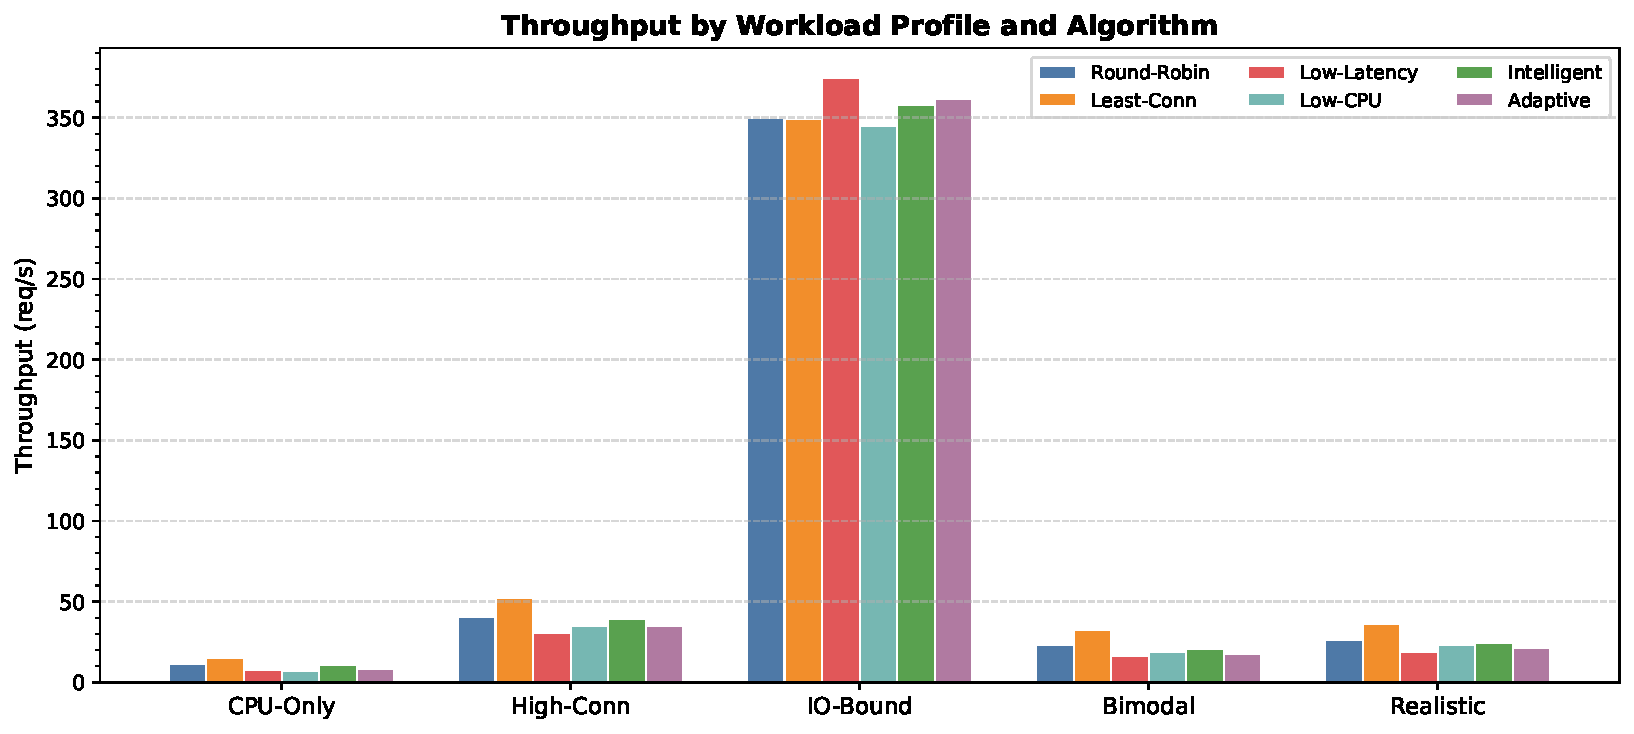
\includegraphics[width=\linewidth]{fig1_throughput_by_profile.pdf}
  \caption{Throughput (req/s) for each algorithm across all five workload profiles.
           Least-connections leads on every CPU-bound profile; all algorithms converge on IO-Bound.}
  \label{fig:throughput}
\end{figure}

\begin{figure}[H]
  \centering
  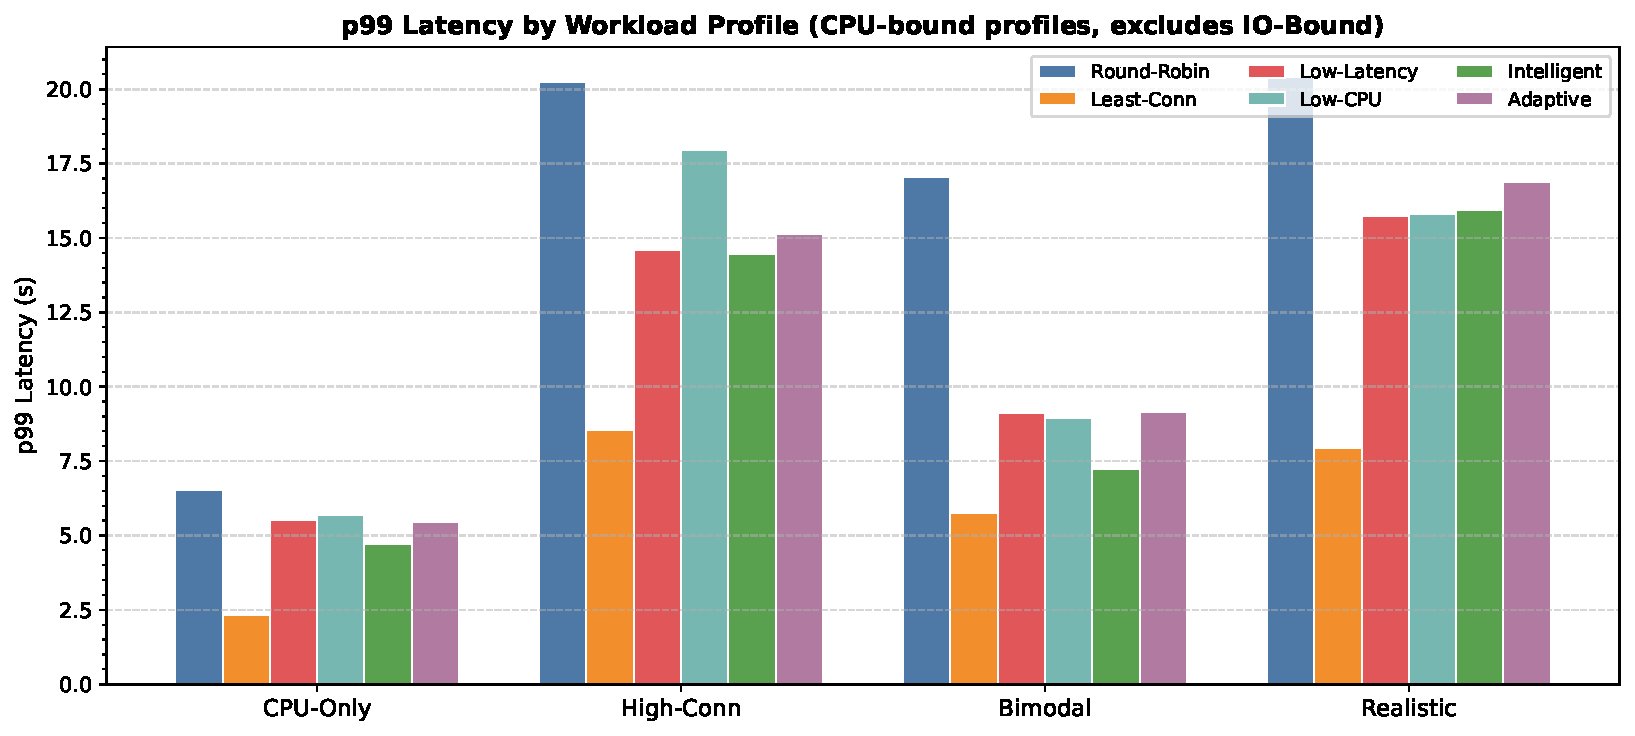
\includegraphics[width=\linewidth]{fig2_p99_by_profile.pdf}
  \caption{p99 latency (seconds) for CPU-bound profiles. Least-connections achieves the lowest
           tail latency by avoiding the saturated weakest backend.}
  \label{fig:p99}
\end{figure}

\paragraph{CPU-bound workloads (cpu\_only, high\_conn, bimodal, realistic).}
Least-connections is the consistent winner. On \texttt{cpu\_only} it achieves
15.4\,req/s versus 11.0 for round-robin (+40\%) and 7.3--7.6 for the
latency-based algorithms. On \texttt{high\_conn} it reaches 52.3\,req/s
versus 40.4 for round-robin (+29\%) and 30.5 for lowest-latency ($-25\%$
relative to round-robin). The mechanism is straightforward: least-connections
implicitly discovers backend capacity by tracking queue depth. Backend-3 (4
vCPU) processes requests faster, drains its connection count sooner, and
therefore attracts proportionally more new requests.

\paragraph{I/O-bound workloads.}
All algorithms converge to $\sim$350\,req/s because compute is not the
bottleneck — the fixed 250\,ms sleep dominates every response regardless of
which backend handles it. Lowest-latency gains a marginal edge (374\,req/s)
by preferring the geographically closest backend, which adds no compute delay.

\paragraph{Network proximity bias.}
Lowest-latency routes 59--96\% of CPU-only traffic to backend-1 (westus2,
1 vCPU) across all profiles. This is the geographically closest backend and
therefore measures the lowest observed RTT, but it is also the most
compute-constrained. The algorithm mistakes network proximity for overall
efficiency, routing the majority of CPU-intensive work to the slowest backend
and achieving throughput 31\% below round-robin on \texttt{cpu\_only}.

\paragraph{Intelligent and adaptive.}
Both algorithms land between round-robin and least-connections on CPU-heavy
profiles. They avoid the worst of the proximity bias but do not fully exploit
the capacity asymmetry that least-connections discovers through its queue-depth
signal. The adaptive algorithm is slightly worse than intelligent on most
profiles, likely because the 30-second weight recomputation cycle means it
spends much of the 90-second run period with stale weights.

\begin{figure}[H]
  \centering
  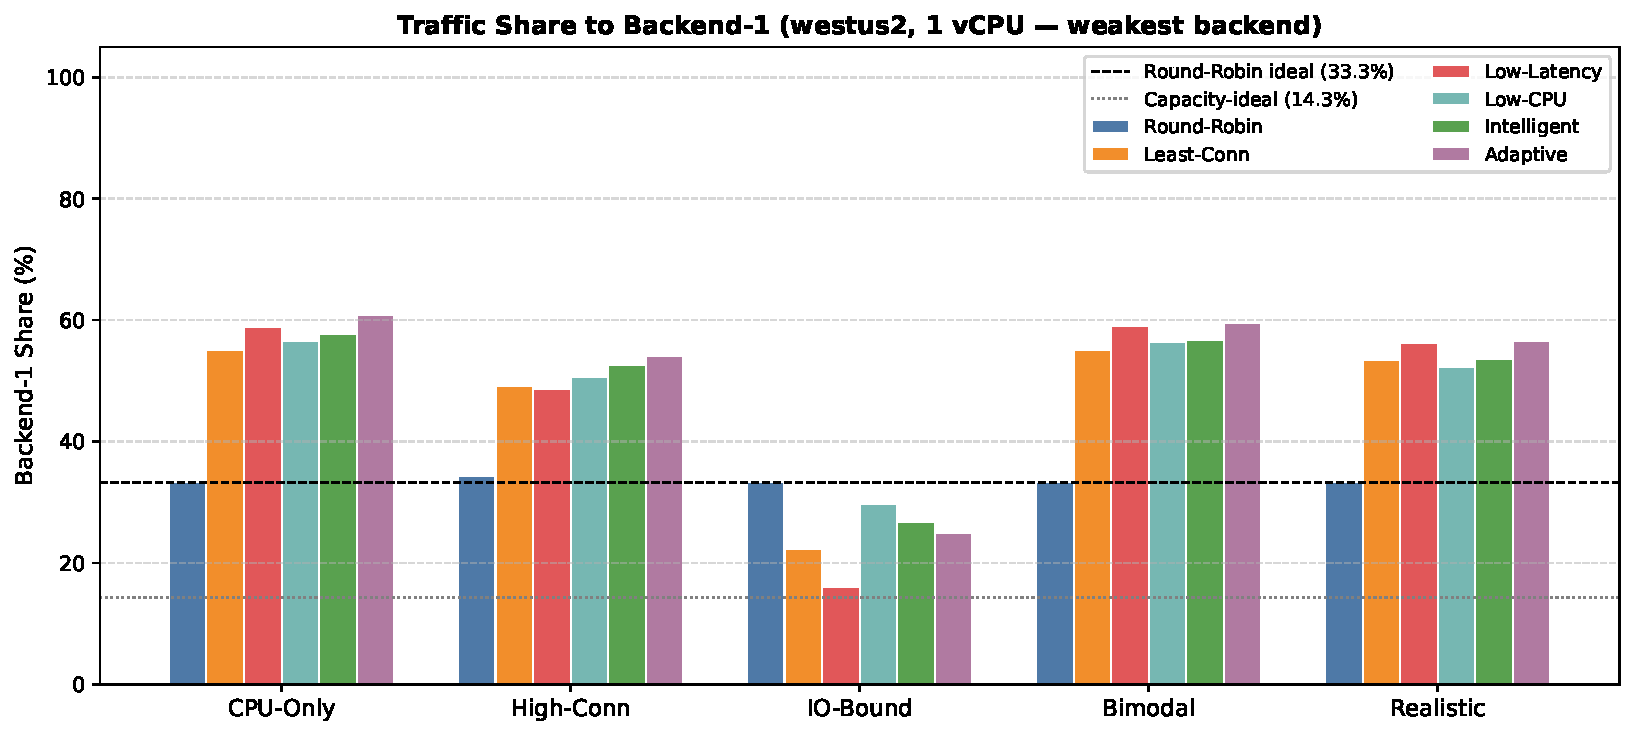
\includegraphics[width=0.85\linewidth]{fig3_b1_share_by_profile.pdf}
  \caption{Fraction of requests routed to backend-1 (westus2, 1 vCPU — weakest and closest).
           Lowest-latency concentrates 59--96\% of traffic there; round-robin holds the 33\% ideal.}
  \label{fig:b1share}
\end{figure}

\subsection{Backend Traffic Distribution}

Table~\ref{tab:dist} shows how each algorithm distributes requests across
backends on the \texttt{cpu\_only} profile. The capacity-proportional ideal
would be 1:2:4 (b1:b2:b3), corresponding to 14\%:29\%:57\%.

\begin{table}[H]
\centering
\begin{tabular}{lrrr}
\toprule
Algorithm & b1 (1 vCPU) & b2 (2 vCPU) & b3 (4 vCPU) \\
\midrule
round\_robin       & 33.3\% & 33.3\% & 33.3\% \\
least\_connections & 50.3\% & 23.6\% & 26.1\% \\
lowest\_latency    & 96.0\% & 0.0\%  & 4.0\% \\
lowest\_cpu        & 63.6\% & 25.3\% & 11.1\% \\
intelligent        & 62.0\% & 17.4\% & 20.6\% \\
adaptive           & 81.5\% & 11.0\% & 7.6\% \\
\bottomrule
\end{tabular}
\caption{Backend request distribution on \texttt{cpu\_only}. Capacity-ideal is
14\%:29\%:57\%. No algorithm achieves this; least-connections comes closest
while still over-routing to b1.}
\label{tab:dist}
\end{table}

\begin{figure}[H]
  \centering
  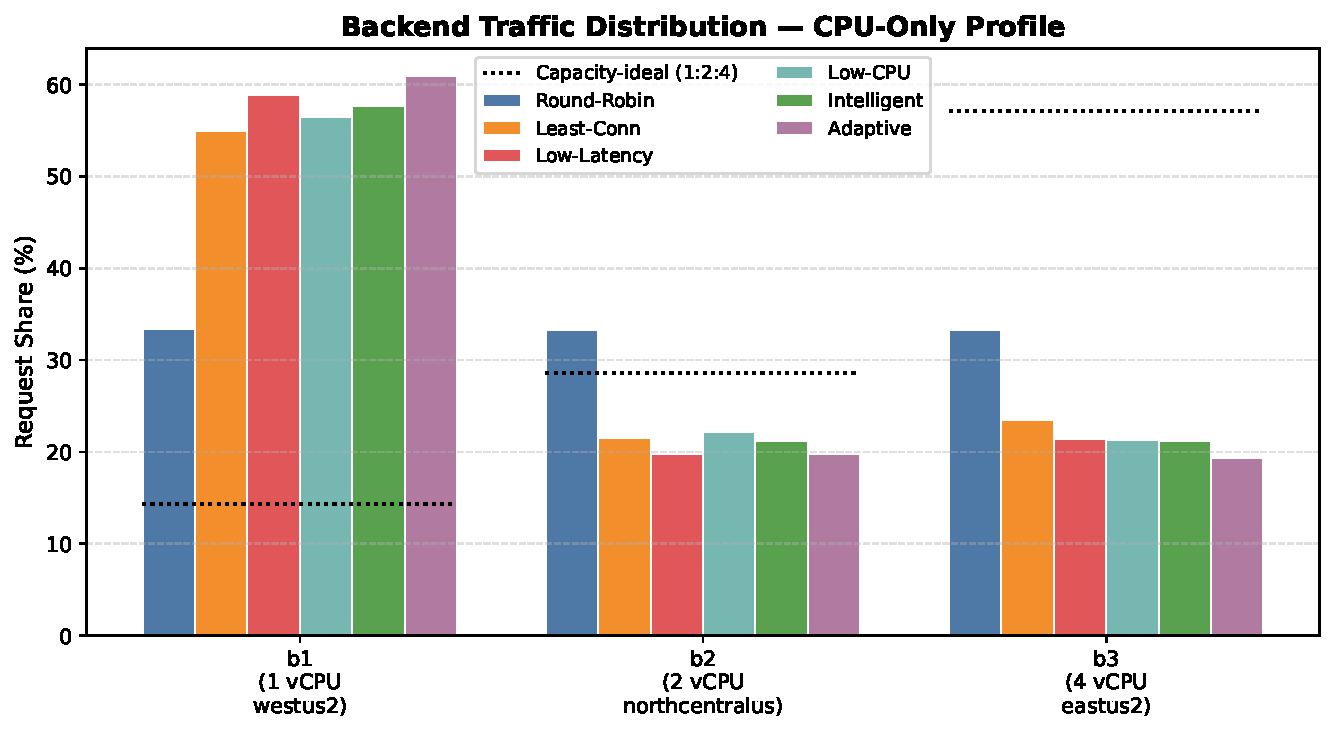
\includegraphics[width=0.85\linewidth]{fig7_backend_dist_cpu_only.pdf}
  \caption{Per-backend request share on the CPU-Only profile. Dotted lines show the
           capacity-ideal 1:2:4 distribution. No algorithm achieves it; lowest-latency
           concentrates almost all traffic on backend-1.}
  \label{fig:dist}
\end{figure}

None of the algorithms achieve the capacity-ideal distribution. Least-connections
over-routes to b1 because the 1-vCPU backend drains its queue between bursts;
during those idle moments its connection count drops to zero and it appears
equally attractive as the larger backends. The metric-based algorithms over-route
to b1 for a different reason: b1 is closest to the client, so it observes lower
raw RTT, which biases latency-normalisation.

\subsection{Saturation Ramp}

Table~\ref{tab:sat} shows the open-loop saturation ramp at intensity=1 with
rates calibrated to bracket the hardware ceiling. The saturation point is
defined as the lowest rate where error rate exceeds 1\% or p99 exceeds
5{,}000\,ms.

\begin{table}[H]
\centering
\small
\begin{tabular}{lrrrrr}
\toprule
Algorithm & Sat. point & p50 @ sat. & p99 @ sat. & err\% @ sat. \\
\midrule
least\_connections & \textbf{150 req/s} & 11{,}306\,ms & 39{,}743\,ms & 35.9\% \\
round\_robin       & 100 req/s & 1{,}547\,ms  & 32{,}917\,ms & 16.4\% \\
intelligent        & 75 req/s  & 1{,}669\,ms  & 10{,}596\,ms & 0.0\% \\
lowest\_latency    & 50 req/s  & 142\,ms      & 19{,}344\,ms & 0.0\% \\
lowest\_cpu        & 50 req/s  & 2{,}267\,ms  & 8{,}137\,ms  & 0.0\% \\
adaptive           & 10 req/s* & 71\,ms       & 52{,}113\,ms & 0.0\% \\
\bottomrule
\end{tabular}
\caption{Saturation ramp results (intensity=1, open-loop, 60\,s per step).
*Adaptive's 10\,req/s trigger is a p99 spike caused by a cold-start weight
recomputation at $t=30$\,s rather than true saturation.}
\label{tab:sat}
\end{table}

\begin{figure}[H]
  \centering
  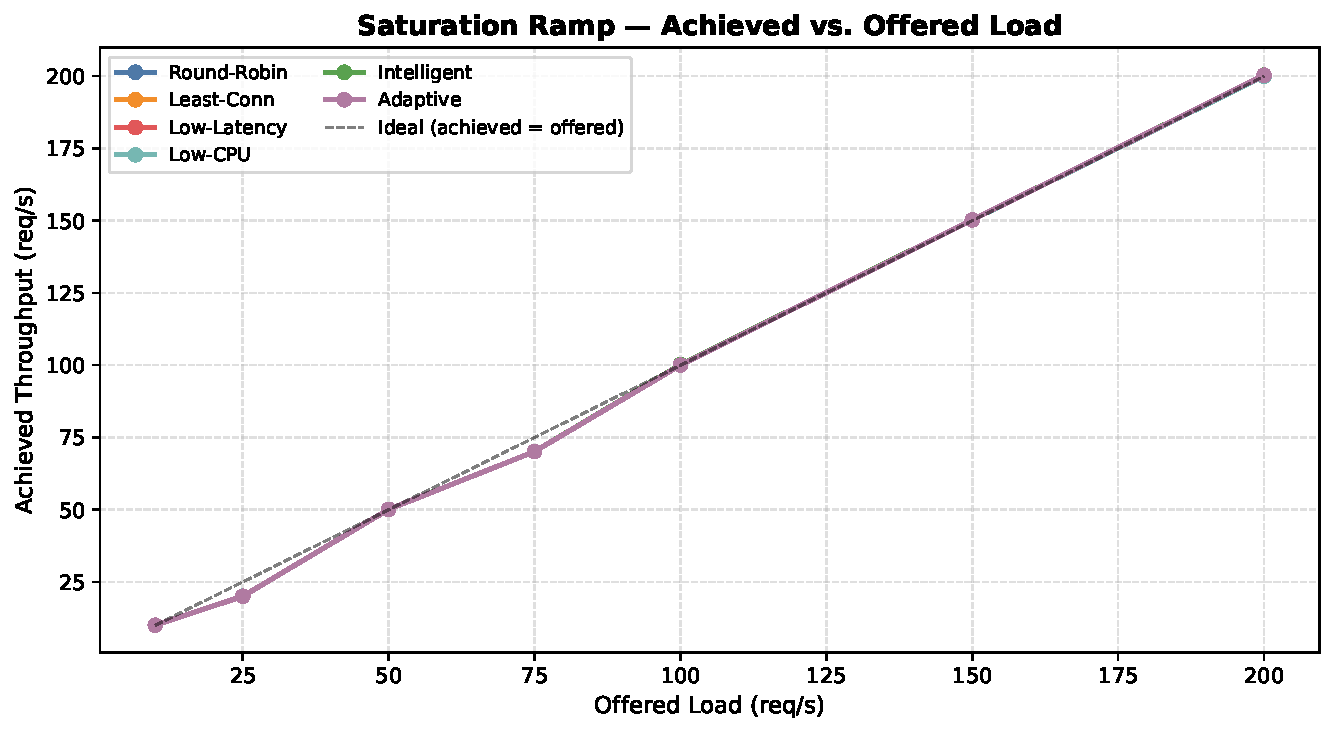
\includegraphics[width=0.85\linewidth]{fig4_saturation_throughput.pdf}
  \caption{Achieved throughput vs.\ offered load. Least-connections tracks the ideal
           line the longest; metric-based algorithms diverge earlier.}
  \label{fig:sat_tput}
\end{figure}

\begin{figure}[H]
  \centering
  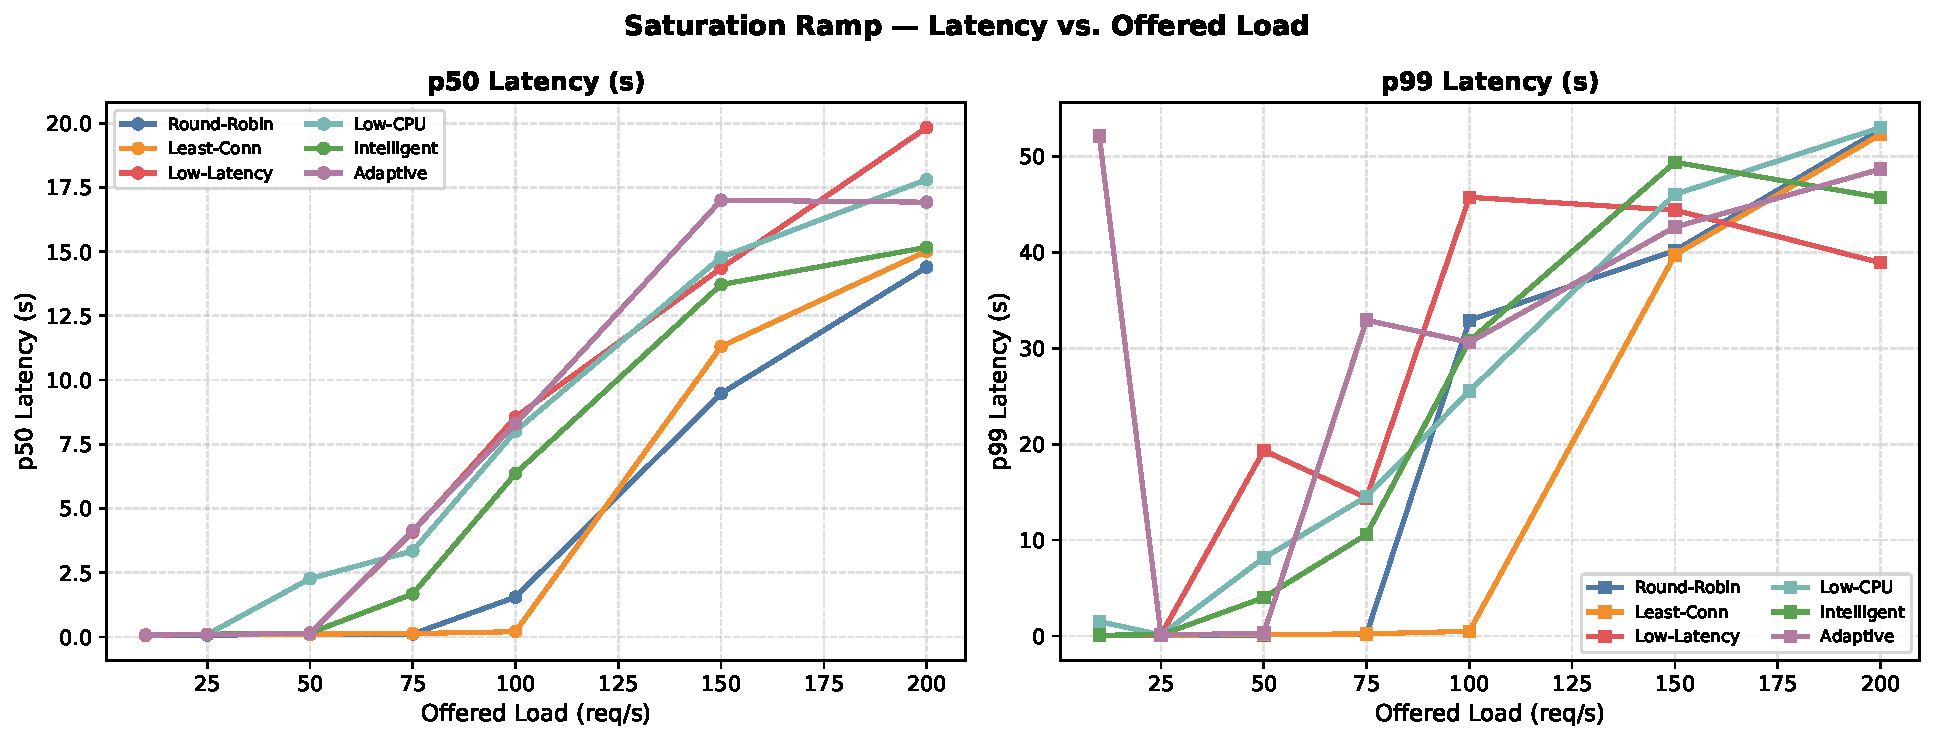
\includegraphics[width=\linewidth]{fig5_saturation_latency.pdf}
  \caption{p50 and p99 latency vs.\ offered load. Latency stays flat until the
           saturation knee, then rises sharply.}
  \label{fig:sat_lat}
\end{figure}

\begin{figure}[H]
  \centering
  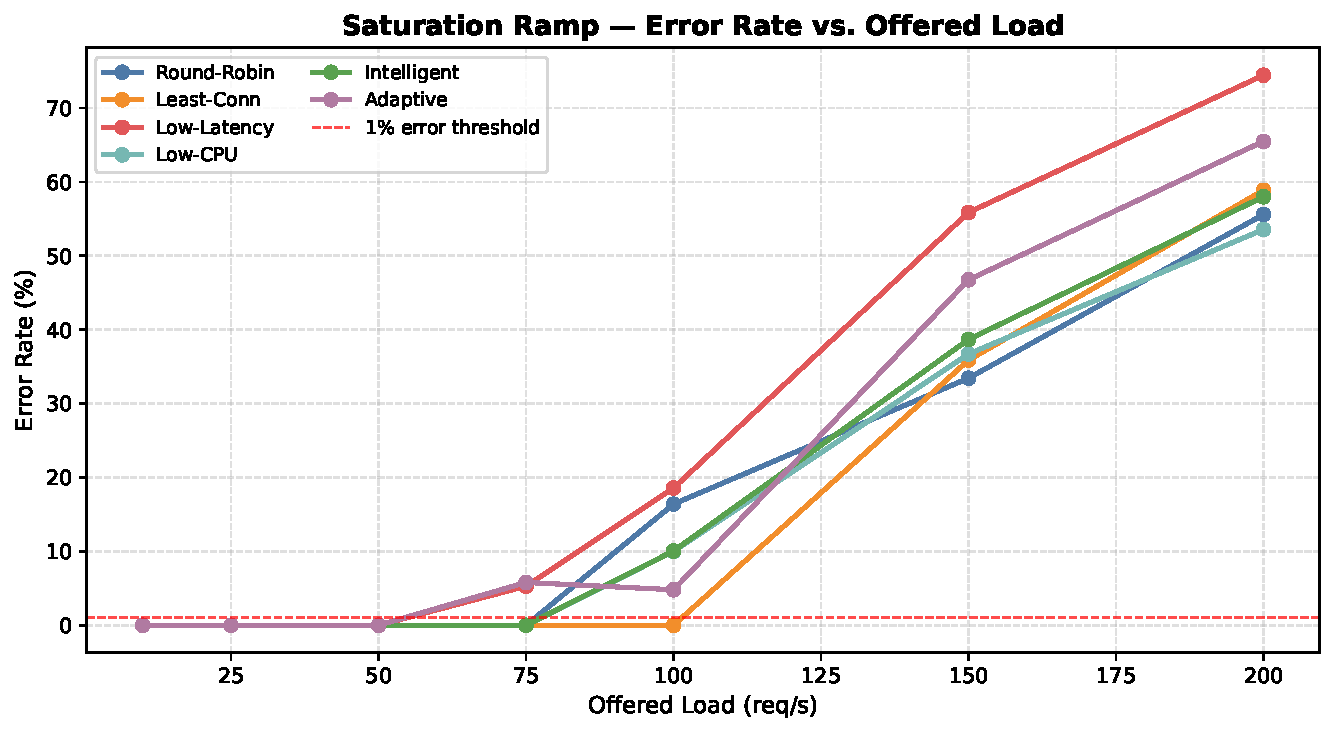
\includegraphics[width=0.85\linewidth]{fig6_saturation_errors.pdf}
  \caption{Error rate vs.\ offered load. The 1\% threshold (dashed red) marks the
           effective saturation point for each algorithm.}
  \label{fig:sat_err}
\end{figure}

Least-connections sustains clean operation up to 100\,req/s (where round-robin
already shows 16\% errors) and does not saturate until 150\,req/s. This is
consistent with its ability to dynamically discover that backend-3 can absorb
more load.

The adaptive algorithm's p99 spike at 10\,req/s is an artifact: the very first
weight recomputation fires at $t=30$\,s, and the resulting routing shift causes
a burst of requests to queue on a newly preferred backend whose metrics have
not yet stabilised. This is a cold-start artefact, not a capacity limit, but
it is flagged by the saturation detector.

% ─────────────────────────────────────────────────────────────────────────────
\section{Deliverables: Building and Running the Project}

\subsection{Repository Structure}

\begin{lstlisting}
inteliLB/
  cmd/
    loadbalancer/   # LB binary (HTTP reverse proxy + algorithm hot-swap)
    backend/        # Backend server (CPU + I/O work, /metrics, /health)
    client/         # Load generator (closed-loop and open-loop modes)
  internal/lb/
    algorithms.go   # All 6 selectors + factory
    algorithms_test.go
    balancer.go     # Balancer core, health-check loop, metrics polling
    backend.go      # Backend struct (atomic counters, EMA latency)
  scripts/
    deploy.sh                     # Azure VM provisioning
    azure/
      launch.sh                   # Per-region VM create + bootstrap
      teardown.sh                 # Resource group deletion
    run-workload-sweep-azure.sh   # Full experiment orchestration
  results/                        # CSV and JSON output from all runs
  report.tex                      # This document
\end{lstlisting}

\subsection{Build}

Requires Go 1.21+.

\begin{lstlisting}[language=bash]
git clone https://github.com/zemanovic/inteliLB
cd inteliLB
go build -o bin/loadbalancer ./cmd/loadbalancer
go build -o bin/backend      ./cmd/backend
go build -o bin/client       ./cmd/client
go test ./internal/lb/ -race   # unit tests
\end{lstlisting}

\subsection{Running Locally}

\begin{lstlisting}[language=bash]
# Start two backend instances on ports 9001 and 9002
./bin/backend -port=9001 &
./bin/backend -port=9002 &

# Start the load balancer
./bin/loadbalancer \
  -port=8080 \
  -algorithm=intelligent \
  -backends=http://localhost:9001,http://localhost:9002

# Run closed-loop load (20 workers, 30s, CPU-only intensity=5)
./bin/client \
  -url=http://localhost:8080 \
  -workers=20 -duration=30s -intensity=5 -mix=cpu:100

# Switch algorithm at runtime
curl -X POST http://localhost:8080/lb/algorithm \
  -H "Content-Type: application/json" \
  -d '{"algorithm":"least_connections"}'
\end{lstlisting}

\subsection{Reproducing the Azure Experiments}

Requires Azure CLI logged in (\texttt{az login}) and an SSH key pair.

\begin{lstlisting}[language=bash]
# Full sweep: 5 workload profiles + recalibrated saturation ramp
./scripts/run-workload-sweep-azure.sh --key-file ~/.ssh/id_rsa

# Saturation ramp only (skips profile sweep)
./scripts/run-workload-sweep-azure.sh \
  --key-file ~/.ssh/id_rsa --saturation-only

# Re-use existing VMs (skip deploy)
./scripts/run-workload-sweep-azure.sh \
  --key-file ~/.ssh/id_rsa --skip-deploy
\end{lstlisting}

Results are written to \texttt{results/\$(date)\_workload\_sweep\_azure/} and
a human-readable summary to \texttt{summary.txt} in that directory. Azure
infrastructure is torn down automatically on script exit.

% ─────────────────────────────────────────────────────────────────────────────
\section{Conclusions and Future Work}

\subsection{Lessons Learned}

\paragraph{Least-connections is remarkably effective for free.}
The single most impactful insight from this project is that tracking in-flight
request count — a zero-overhead signal available without any polling — yields
consistently superior throughput on CPU-bound workloads across every profile
tested. It outperforms algorithms that have access to explicit CPU\% and latency
measurements, because the connection count serves as an implicit capacity
signal: a backend that processes requests faster always has fewer active
connections.

\paragraph{Network proximity dominates latency-based routing.}
Cross-region RTT variation (westus2 $\approx$ 30--60\,ms, northcentralus
$\approx$ 40--70\,ms, eastus2 $\approx$ 50--90\,ms from the test client)
overwhelms the compute-latency differences on lightly loaded backends. Routing
to the closest region maximises I/O-bound throughput but severely penalises
CPU-bound throughput by over-loading the weakest backend.

\paragraph{Multi-metric scoring needs better feature engineering.}
The intelligent and adaptive algorithms use raw metric values. Because
latency includes network RTT, the geographically close backend always has
lower normalised latency regardless of compute load, biasing the weighted
score toward the same backend that lowest-latency would choose. Subtracting
a network baseline (e.g., ICMP RTT to each backend) from measured response
latency before scoring would isolate compute-attributable latency and
likely produce a more useful signal.

\paragraph{Cold-start and weight recomputation timing matter.}
The adaptive selector's 30-second recomputation cycle is misaligned with the
90-second experiment window: it fires once per run, causing a visible routing
shift mid-experiment. A shorter interval (5--10\,s) with rate-limiting on
large weight changes would smooth this out.

\paragraph{Open-loop clients must use context cancellation for safe drain.}
Early iterations of the load generator used a \texttt{select} between a
results channel and a \texttt{drainDone} channel to unblock in-flight goroutines
after the deadline. This has an unavoidable race: when both cases are
simultaneously ready, Go selects randomly, meaning goroutines can write to a
closed channel. The correct fix is passing a \texttt{context.WithCancel} to
\texttt{http.NewRequestWithContext}: cancelling the context aborts all in-flight
HTTP requests, \texttt{wg.Wait()} completes deterministically, and
\texttt{close(results)} is then safe.

\subsection{What Remains}

\begin{itemize}
  \item \textbf{Network-adjusted scoring:} Subtract per-backend ICMP RTT
        baseline from measured latency to isolate compute latency.
  \item \textbf{Weighted round-robin:} Assign static weights proportional to
        vCPU count. This would route 57\% of traffic to backend-3 from the
        start, requiring no metrics polling and likely outperforming all
        current algorithms on CPU-bound workloads.
  \item \textbf{Request shadowing / canary:} Send a fraction of requests to
        all backends to maintain live metric estimates even when a backend
        receives little organic traffic.
  \item \textbf{Faster adaptive reweighting:} Shorten the recomputation interval
        to 5\,s and add exponential smoothing to prevent weight oscillation.
  \item \textbf{TLS and HTTP/2:} Current implementation is HTTP/1.1 only.
\end{itemize}

\subsection{Connection to CS640 Material}

This project directly exercises core CS640 topics. The load balancer is
fundamentally a layer-7 routing system, and the algorithm comparison is an
empirical study of how routing policy affects end-to-end latency and throughput
in a WAN-scale deployment. The proximity bias observed in lowest-latency routing
reflects the same tension between link-state shortest-path routing and
traffic-aware routing studied in the context of OSPF and SDN. The adaptive
weight recomputation is conceptually similar to congestion-signal-based
algorithms (DCTCP, BBR) in that it adjusts behaviour based on observed
network and system state rather than static configuration.

% ─────────────────────────────────────────────────────────────────────────────
\begin{thebibliography}{9}

\bibitem{nginx}
NGINX Inc. \textit{NGINX Load Balancing}. 2024.
\url{https://docs.nginx.com/nginx/admin-guide/load-balancer/http-load-balancer/}

\bibitem{haproxy}
HAProxy Technologies. \textit{HAProxy Configuration Manual}. 2024.
\url{https://www.haproxy.com/documentation/}

\bibitem{consistent-hashing}
D.~Karger et al. \textit{Consistent Hashing and Random Trees: Distributed
Caching Protocols for Relieving Hot Spots on the World Wide Web}. STOC 1997.

\bibitem{power-of-two}
M.~Mitzenmacher. \textit{The Power of Two Choices in Randomized Load
Balancing}. IEEE Transactions on Parallel and Distributed Systems, 2001.

\bibitem{join-idle-queue}
Y.~Lu, Q.~Xie, G.~Kliot, A.~Geller, J.~Larus, A.~Greenberg. \textit{Join-Idle-Queue:
A Novel Load Balancing Algorithm for Dynamically Scalable Web Services}.
Performance Evaluation, 2011.

\bibitem{maglev}
D.~Eisenbud et al. \textit{Maglev: A Fast and Reliable Software Network Load
Balancer}. NSDI 2016.

\bibitem{go-concurrency}
A.~Donovan, B.~Kernighan. \textit{The Go Programming Language}. Addison-Wesley,
2015.

\end{thebibliography}

\end{document}
